
\chapter{Design in reaction to CDCS}

From its very inception, Skedge's functionality and visual design were driven by the shortcomings of CDCS. It was built \emph{bottom-up}, not \emph{top-down}---every aspect of the application was either made as a reaction to a particular grievance in CDCS or as the natural evolution of an existing feature. Skedge is thus rooted in \emph{usability} derived from real need, not mere conjecture along the question ``what could students want?''. Its success with students, shown in Chapter 4, demonstrates that this usability extends beyond my own standard and can fulfill the various discovered use-cases of students in general.

In this chapter, I will

%%%

\section{Modernity}

CDCS is an old system, relatively speaking, and its recent development has been stagnant. It launched in 2009, seven years ago, and has hardly changed since. Figure \ref{fig:cdcs2010} shows CDCS in July 2010, which, besides the addition of a few search fields, is identical to its current version. Since its introduction in 2009, we have seen the rise of mobile devices into ubiquity, a boom in ``hacker culture'' and public APIs, and the capability for standalone web applications to be as sophisticated and dynamic as desktop-class applications without the aid of browser extensions.

\begin{figure}[ht]
  \centering
    \fbox{
      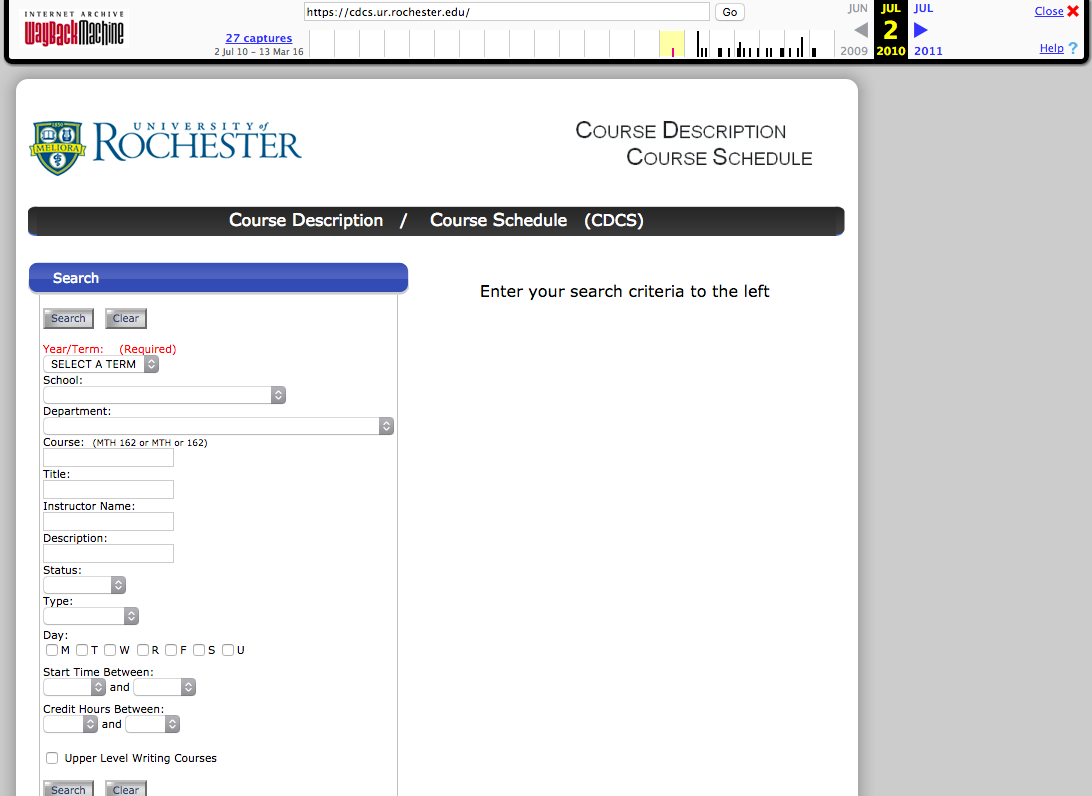
\includegraphics[width=10cm]{images/cdcs/2010}
    }
  \caption{CDCS in July 2, 2010, courtesy of \emph{Archive.org}}
  \label{fig:cdcs2010}
\end{figure}

\subsection{Mobile}

- Important nowadays

- Mobile traffic stat or smth

\begin{figure}[ht]
  \centering
  \begin{tabular}{c c}
    \begin{subfigure}[h]{4cm}
      \centering
      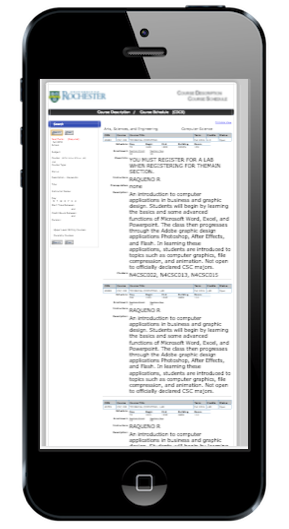
\includegraphics[width=1.00\textwidth]{images/cdcs/mobile}
      \caption{CDCS} \label{fig:cdcs-mobile}
    \end{subfigure}
    \begin{subfigure}[h]{3.9cm}
      \centering
      
\includegraphics[width=1.00\textwidth]{images/skedge/mobile}
      \caption{Skedge} \label{fig:sk-mobile}
    \end{subfigure}
  \end{tabular}
  \caption{CDCS and Skedge running on a mobile device}
\end{figure}

\subsection{Public API}

With the increasing number of attendees at University of Rochester's hackathons, it is clear that the University's ``hacker culture'' is growing (e.g. more students collaborating to build side-projects that integrate resources and servies often benefitting the student community), and projects that include the University's course catalog are becoming more common. Open-source and open-information services greatly help to foster such innovation, and having public APIs is essential toward this end.

Skedge provides a public JSON API at the root URL \url{http://www.skedgeur.com/api/}, made at the request of a student that was interested in using its course data, and the API has already been used in projects by several other student groups. The endpoints included are \url{/api/courses?q=query} (Skedge's query language---described in detail in section 2.3---is supported here), \url{/api/departments?q=optional_query}, and \url{/api/instructors?q=optional_query}.

\subsection{Built-in scheduler vs. browser extension}

- Better UX

- Data is centralized

\subsection{GET requests vs. AJAX}

- Can use back button

- Can send a link to a course or search

%%%

\section{Usability}

\subsection{Data quality}

- Courses don't shout
- Typos in comments
- 12-hour time

\subsection{Section display}

- Grouped course sections
- Embedded labs (A/B too), workshops, \& recitations

- More concise, space efficient (collapsable)
- Eliminates redundancy of same stuff (instructor, description, course title, etc)
- Don't have to pay more attention that you should to whether it's a different course or the same one

Note that in Figure \ref{fig:cdcs-sections}, the first two boxes are sections for the same course, and the next two are labs for that course. Four more lab sections and \emph{twenty} more workshop sessions for that same course follow below the truncated screenshot. Figure \ref{fig:sk-sections} demonstrates how this information can be conveyed more concisely.

\begin{figure}[ht]
  \centering
  \begin{tabular}{c c}
    \begin{subfigure}[h]{6cm}
      \centering
      \fbox{
        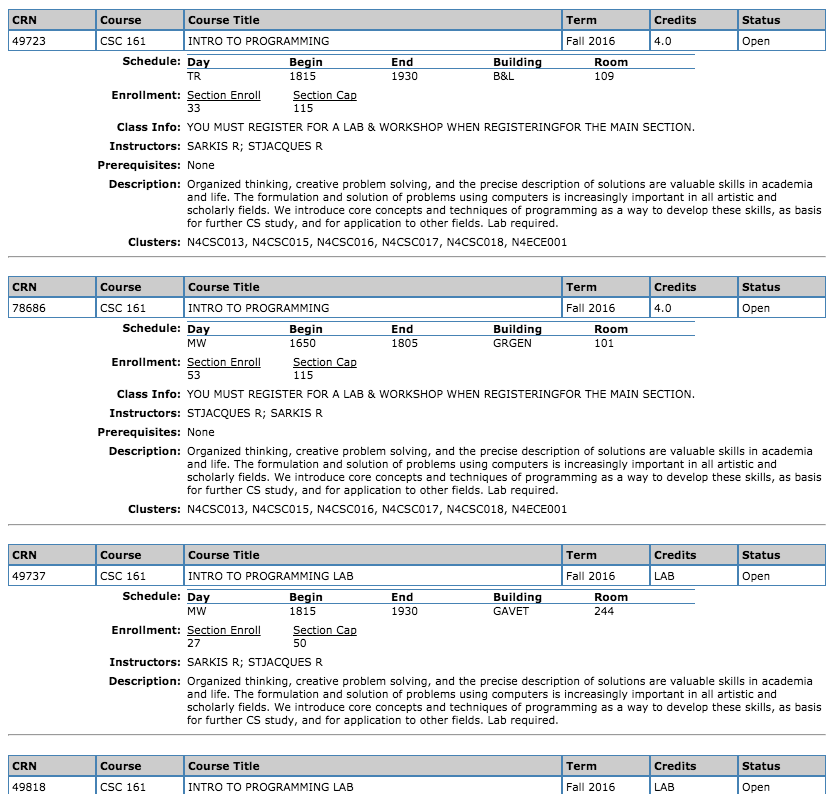
\includegraphics[width=1.00\textwidth]{images/cdcs/sections}
      }
      \caption{Ungrouped sections in CDCS} \label{fig:cdcs-sections}
    \end{subfigure}
    \hspace{15pt}
    \begin{subfigure}[h]{7cm}
      \centering
      \fbox{
        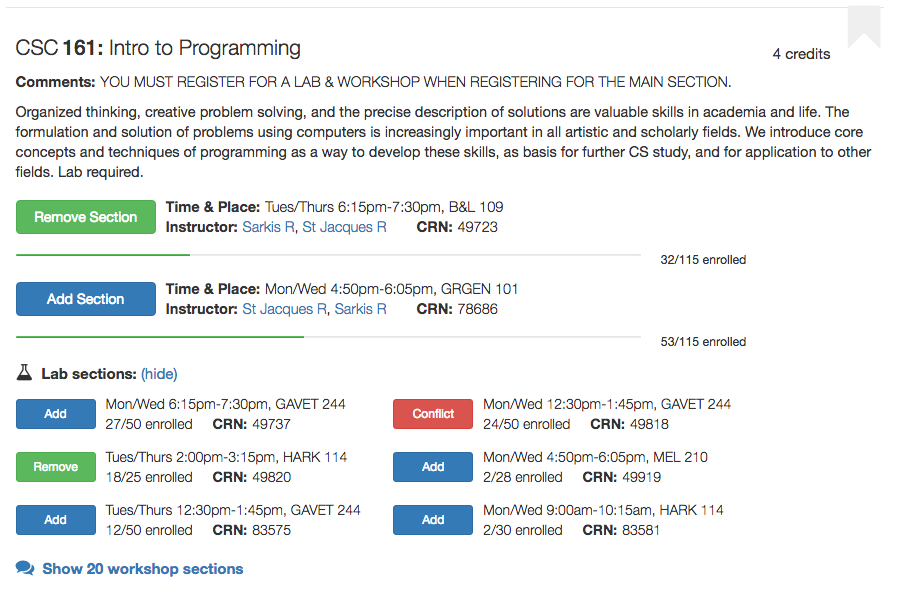
\includegraphics[width=1.00\textwidth]{images/skedge/sections}
      }
      \caption{Grouped sections in Skedge} \label{fig:sk-sections}
    \end{subfigure}
  \end{tabular}
  \caption{Section presentation on CDCS and Skedge}
\end{figure}


\subsection{Course reference}

\begin{figure}[ht]
  \centering
  \fbox{
    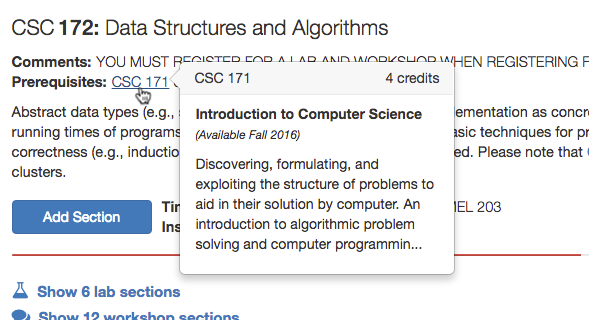
\includegraphics[width=8cm]{images/skedge/hover}
  }
  \caption{Hoverable and clickable course and instructor mentions in Skedge} \label{fig:sk-hover}
\end{figure}

- Clickable/hoverable course links, professor searches

\subsection{Multiple schedule support}

- Old CDCS+betterCDCS system can't keep track of this, have conflicts when adding stuff

\subsection{Exporting to GCal, .ics, image}

- Mobile sync support
- Security: BetterCDCS export gcal is currently broken and sends netID in PLAINTEXT over http(!!!)

\subsection{Search}

Most important usability concern is finding courses.

%%%

\section{Search}

Use cases, natural language.

\subsection{Course selection criteria}

Narrowed it down to three criteria. Keep in mind that \emph{none} of the things listed below are supported by CDCS, and they are all supported by Skedge.

  \subsubsection{Requirements}

  - Finding crosslists
  - Clusters

  \subsubsection{Browsing}

  - ``New'' courses
  - ``Autofit'' search
  - Random
  - Sorts

  \subsubsection{Friends}

  - ``What are my friends taking?'' (``what are you taking this semester'' = probably most common smalltalk phrase uttered on campus)
  - ``What do my friends recommend?'' - ``have you taken this class, and if so, what did you think of it?''

\subsection{Natural language search}

%Figure

See figure.

  \subsubsection{Advantages}

  - 15 fields reduced to 1

  vs form entry:
  - Faster
  - More intuitive
  - More easily extendable

  \subsubsection{Disadvantages}

  Having to know the DSL, grammar ambiguities (can be solved with a `did you mean')

\subsection{Multipurpose}

Used by other links (instructors, course references) around the site

\subsection{Added features}

- CRN (!)
- Crosslist
- Class size

%%%

\section{Social}

\subsection{The issue}

  \subsubsection{Static image vs. live site}

  - Edits don’t update
  - Referencing courses

  \subsubsection{Finding common courses}

  - requires your friends to share their schedules on FB publicly and you to see their post


%%%%%%%%%%%%%%


  - is schedule-first, not search-first
  - typically only occurs for the current semester

%figure

\subsection{Skedge Social}

% Walkthru

  \subsubsection{Friends' course enrollments}

  Mini-feed

  \subsubsection{Friends' course likes}

  \subsubsection{Likes \& enrollments embedded in results}

  \subsubsection{Personal schedule synchronization}

  \subsubsection{Privacy}

  \subsubsection{Notifications}

  %figs of the 2 types